\chapter{システム全体像}
\thispagestyle{myheadings}

\section{全体の流れ}

\subsection{提案手法}
図1に本研究の全体像を示す.

システムの流れはコンテンツを視聴しているときの生体データを取得し、サーバにアップロードする。一つのコンテンツに対したくさんのデータを収集する。集めた生体データから盛り上がっている箇所を推定し、抜き出す。抜き出したデータを基にコンテンツに重畳表示するといった構成である。


\subsection{生体データの分析と心拍上昇箇所の抽出処理}
生体データを観察しその分析と心拍上昇箇所の抽出処理方法を述べる。生体データの収集方法としてスマートウォッチを利用する。今回TicWatchE3を利用した。

この研究では生体データとして心拍数を使用することとした。理由としてスマートウォッチを使い気軽に計測ができるためである。AndroidStudioで心拍数が収集できるアプリを作成した。


記録したデータをサーバにアップロードする。実際に集めたデータをグラフにしたものを表示する。映画は「キングコング」を視聴した人のデータである。


集めたデータを観察したところ人により心拍数の変動が様々であった。映画の盛り上がりのシーンを抜き出すため、心拍数が上昇している箇所を抽出する。収集した心拍数の CSV データを心拍上昇箇所のみのJSON データにする.抽出処理の方法を図 2 に示す.

スマートウォッチで収集した心拍数のデータはcsvファイルとしてサーバにアップロードされる。サーバから一つ一つのデータ毎に心拍数上昇箇所の抽出を行い、上昇した箇所のみのjsonデータにする。処理を行ったデータを最終的に一つのjsonデータに変換する。安静時の心拍数からどれだけ心拍数が上昇したかを抽出するため、まず映画を見る前の1分間を安静時の心拍数として平均を出し閾値にする. 次に図のように心拍 数を閾値と比較する.心拍数の上昇具合で表示するエフェクトを変更するため、1 から 3 までのレベル分けをした.平均心拍数よりも心拍数が 16bpm 以上高い時を レベル 3,14bmp 以上をレベル2,12bpm 以上をレベル 1 とする. from to の形式で心拍数が閾値を超えていた 時間を示す.時間は映画が始まってからの経過時間で エフェクトを表示するため相対時間にした.effectlevel で表示するエフェクトを決定する。

実際に心拍数上昇箇所の抽出処理をした後のデータを載せる。

エフェクトの表示に適した形式にするため、心拍上昇箇所の抽出処理した JSON データを一つの JSON データにまとめる.これにより一つのコンテンツに一個の JSON データが作られる.このデータを使いエフェクトを映画画面に重畳する.

\section{エフェクト表示}

\subsection{エフェクト表示方法}
エフェクト表示方法として,カテゴリやレベルごとにエフェクトを用意し,動画として重畳表示しているが,レベル分けを行ったためエフェクトをダイナミックに生成できず,細かな心拍数変化を表示できていない.
本研究では,視聴者ごとにエフェクトを自由に選択できるようにするためElectronを使用し,PCを使用する環境下での重畳表示が可能になっている.
Electronを起動し,視聴する動画コンテンツを選択し,視聴する映画のジャンルに合わせるエフェクトを選択し,Playをクリックすることでエフェクト重畳が開始するようになっている.
実際の動作画面を図3.1.1に示す.
\begin{figure}[H]
    \centering
    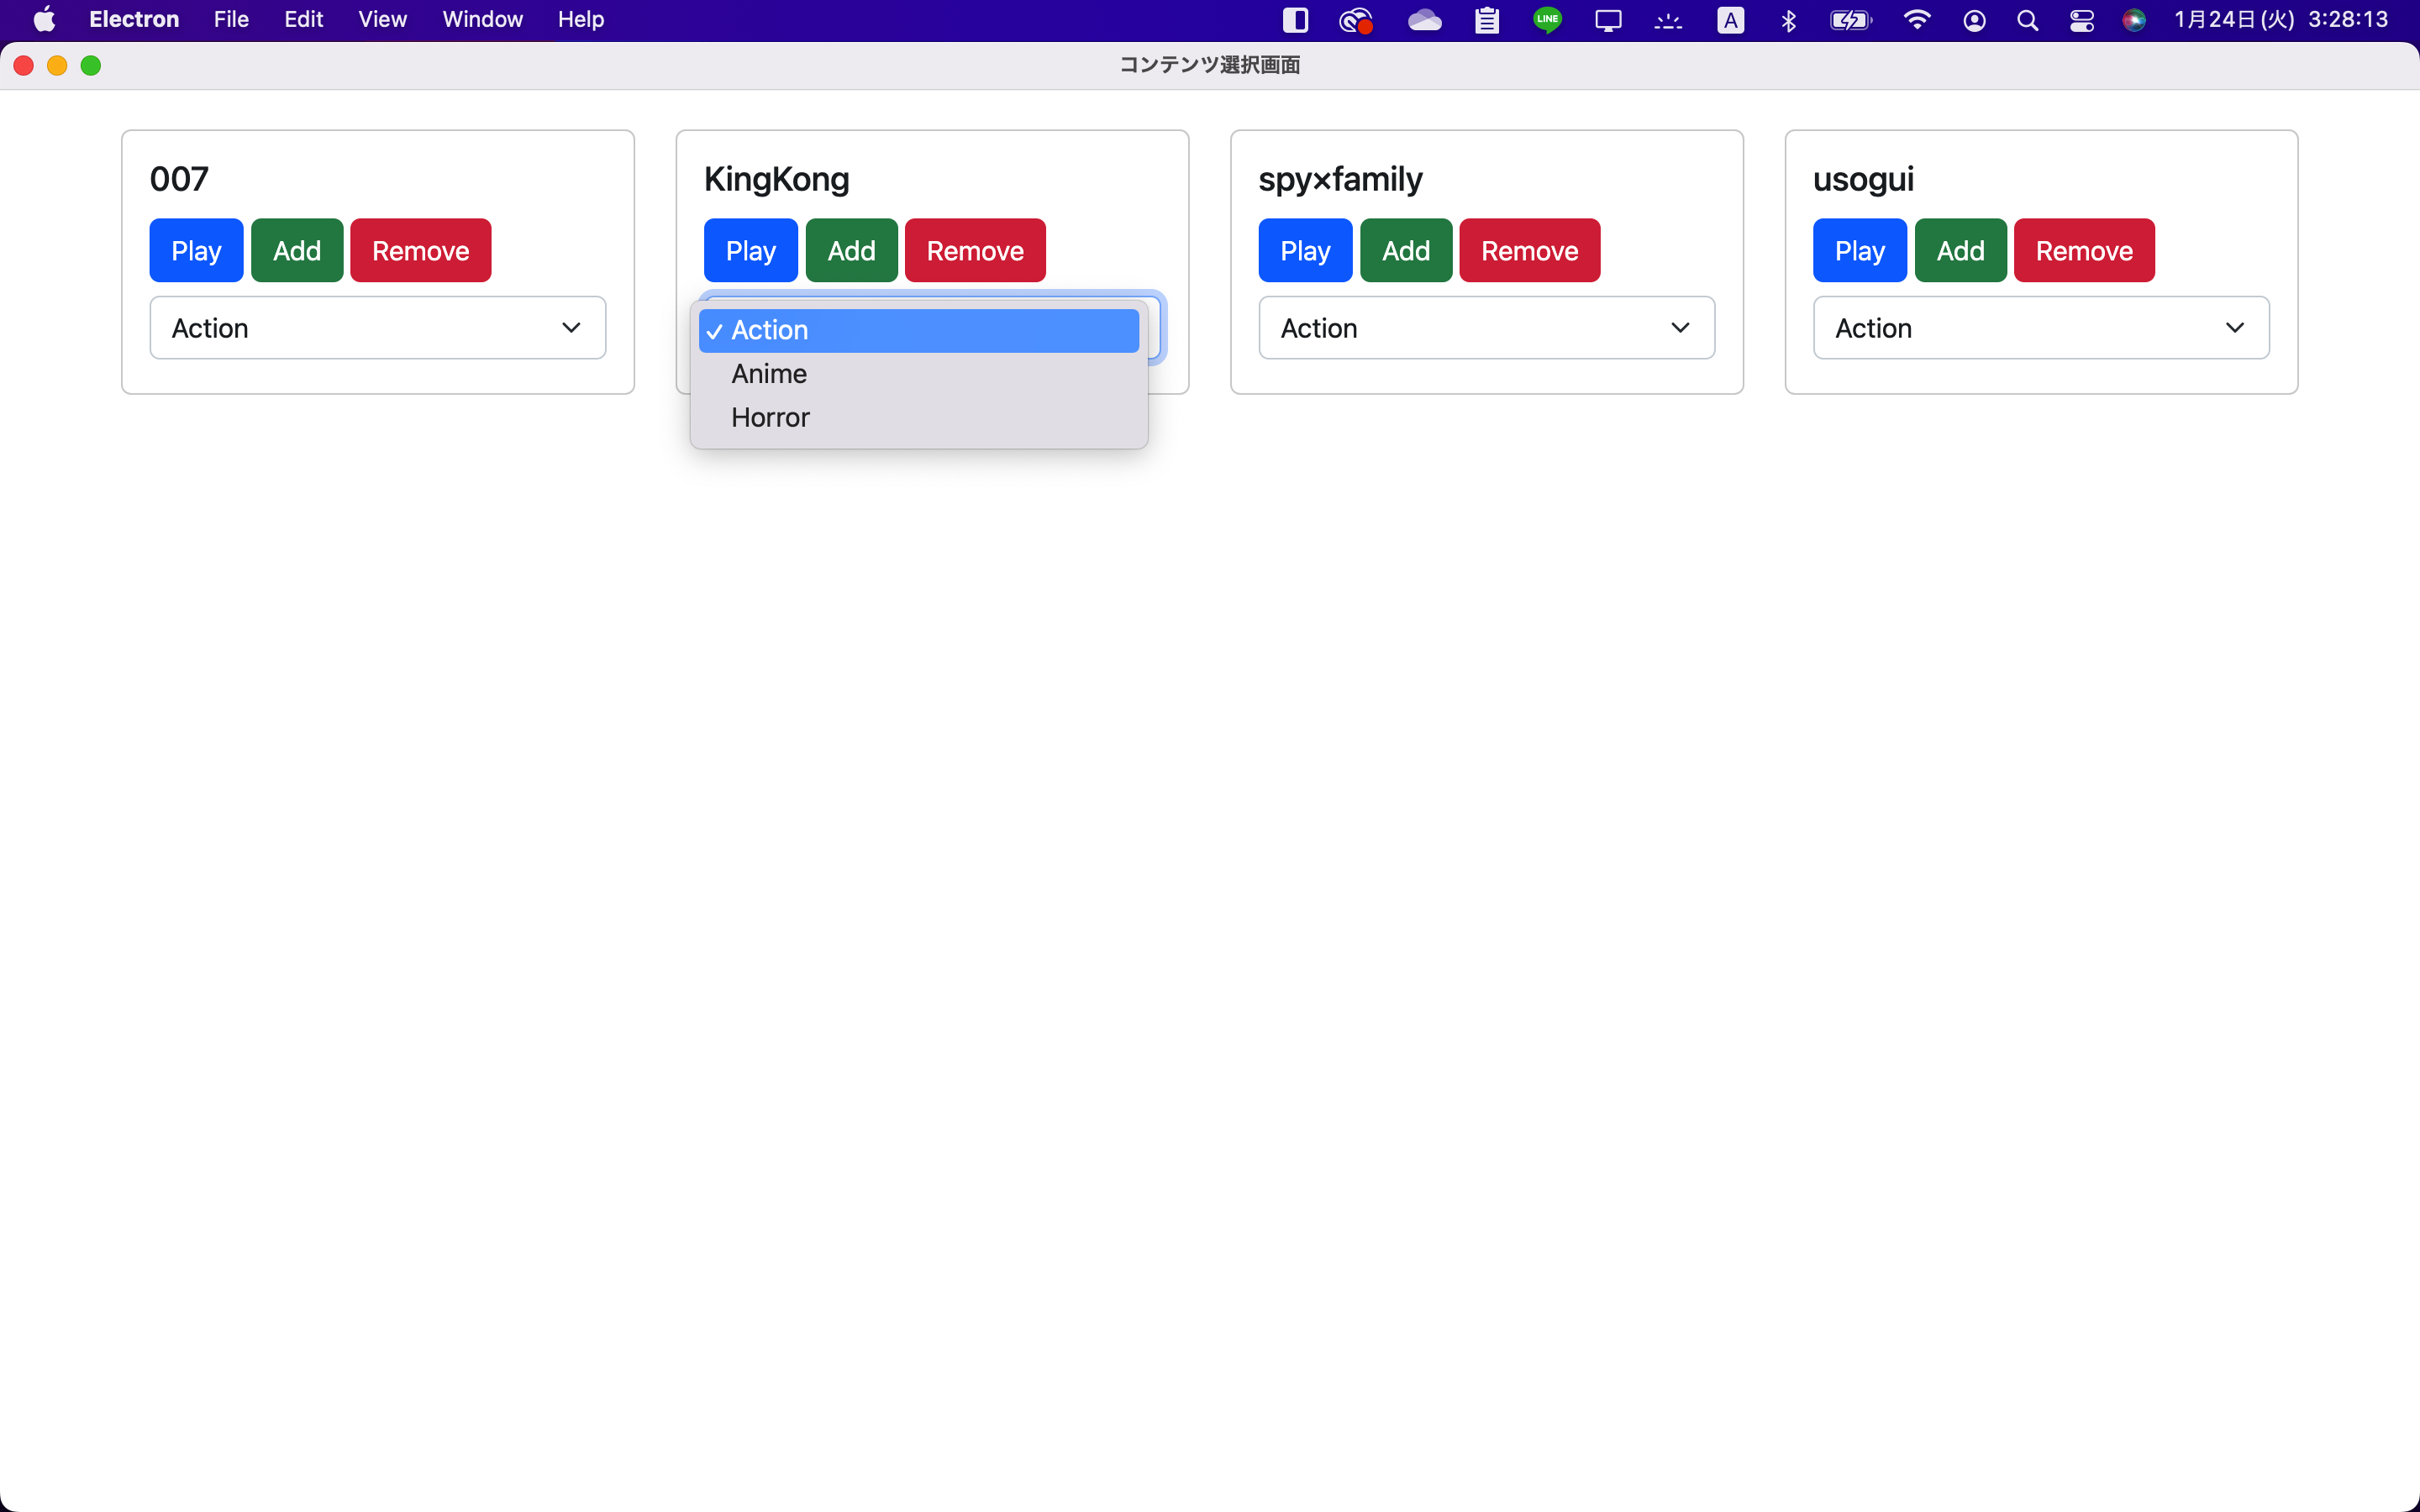
\includegraphics[width=10cm]{images/chapter3/contents.jpg}
    \caption{コンテンツ選択画面}
    \label{abst}
\end{figure}


\subsection{エフェクトの種類}
エフェクトの種類としてAction, Anime, Horrorの3種類に分け見る映画のジャンルを選択可能にした.選択できるようにした理由として,視聴ジャンルによって同じエフェクト効果を表示した際に,エフェクトが映像視聴の際に邪魔になってしまう点が挙げられる.
エフェクトの目的として,Actionのエフェクトは迫力・緊迫感を与え,Animeのエフェクトは面白さを与える.Horrorのエフェクトは恐怖を軽減させる目的として制作した.心拍データの処理の際に1から3までのレベル分けの結果でエフェクトが変更される.1から3に分けた際に1の結果が出力された時間はエフェクトを透過し映像視聴の邪魔にならないように制作し,2と3の結果が出力されている時のみに2段階に分けエフェクトが表示されるように制作した.
実際の画面にエフェクトを表示した例を図3.3.2に示す.Actionのエフェクトは赤色の不透明度を上げ,色相彩度を上げる.Animeのエフェクトは効果線を増やす.Horrorのエフェクトは不透明度を下げ,ぼかしの不透明度を上げるように制作した.Action, Horrorのエフェクト制作ではAfter Effectsを使用しフラクタルノイズ効果.色被り補正で制作.Animeのエフェクト制作ではIllustratorを使用し効果線を制作した.
\begin{figure}[H]
    \centering
    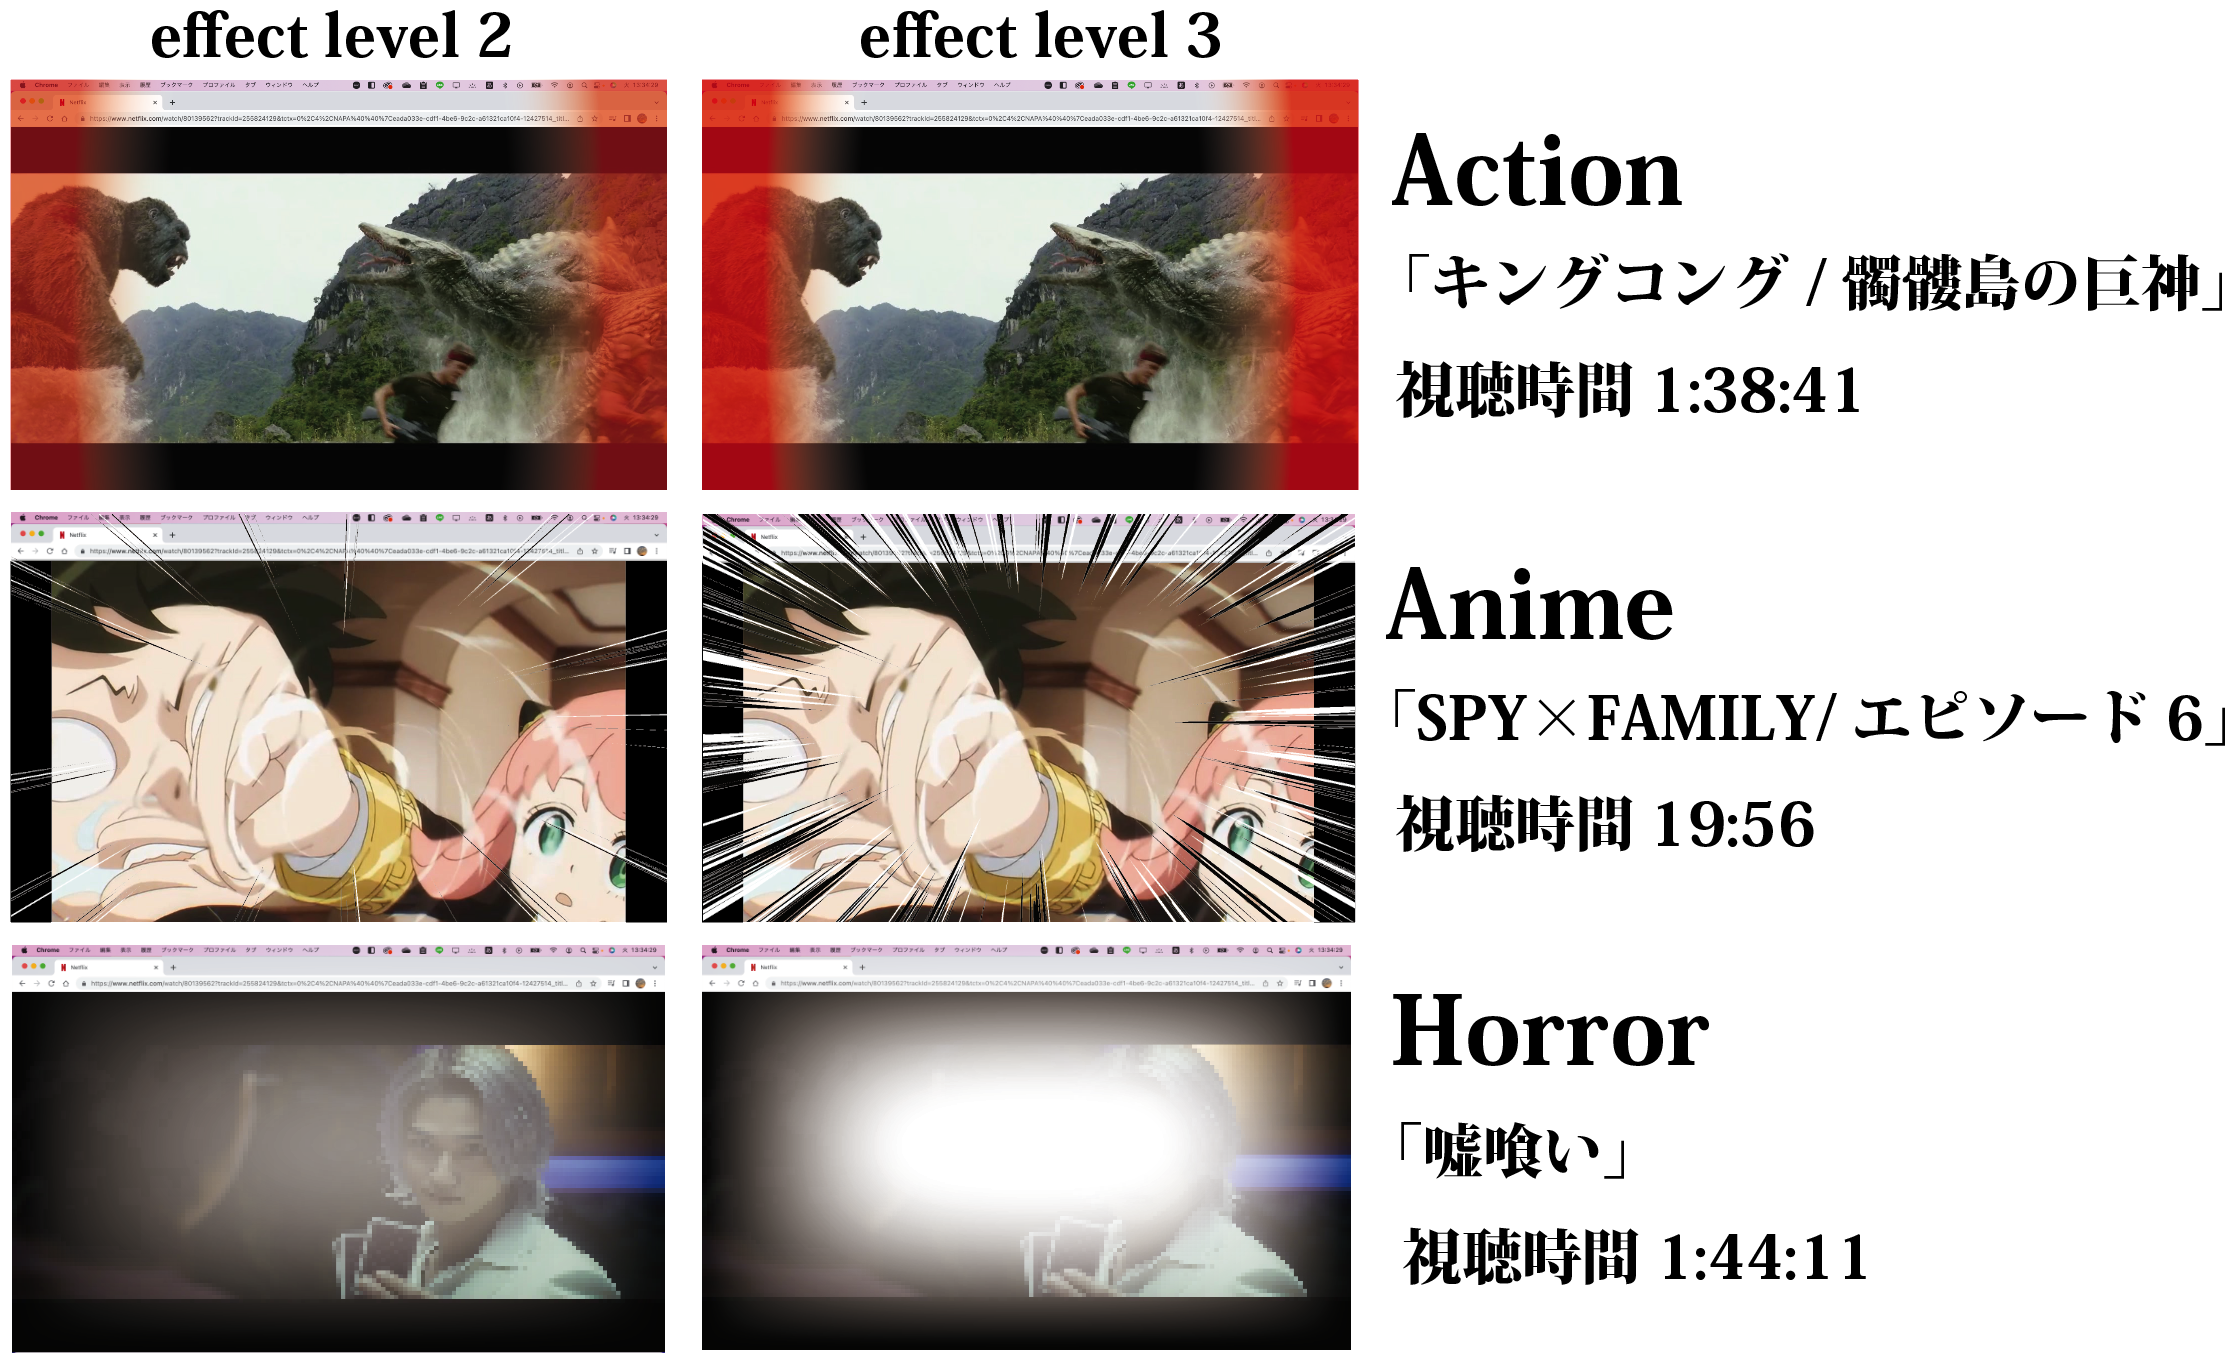
\includegraphics[width=10cm]{images/chapter3/effectjissou.jpg}
    \caption{実装画面}
    \label{abst}
\end{figure}
